\documentclass[twoside]{book}

% Packages required by doxygen
\usepackage{fixltx2e}
\usepackage{calc}
\usepackage{doxygen}
\usepackage[export]{adjustbox} % also loads graphicx
\usepackage{graphicx}
\usepackage[utf8]{inputenc}
\usepackage{makeidx}
\usepackage{multicol}
\usepackage{multirow}
\PassOptionsToPackage{warn}{textcomp}
\usepackage{textcomp}
\usepackage[nointegrals]{wasysym}
\usepackage[table]{xcolor}

% Font selection
\usepackage[T1]{fontenc}
\usepackage[scaled=.90]{helvet}
\usepackage{courier}
\usepackage{amssymb}
\usepackage{sectsty}
\renewcommand{\familydefault}{\sfdefault}
\allsectionsfont{%
  \fontseries{bc}\selectfont%
  \color{darkgray}%
}
\renewcommand{\DoxyLabelFont}{%
  \fontseries{bc}\selectfont%
  \color{darkgray}%
}
\newcommand{\+}{\discretionary{\mbox{\scriptsize$\hookleftarrow$}}{}{}}

% Page & text layout
\usepackage{geometry}
\geometry{%
  a4paper,%
  top=2.5cm,%
  bottom=2.5cm,%
  left=2.5cm,%
  right=2.5cm%
}
\tolerance=750
\hfuzz=15pt
\hbadness=750
\setlength{\emergencystretch}{15pt}
\setlength{\parindent}{0cm}
\setlength{\parskip}{3ex plus 2ex minus 2ex}
\makeatletter
\renewcommand{\paragraph}{%
  \@startsection{paragraph}{4}{0ex}{-1.0ex}{1.0ex}{%
    \normalfont\normalsize\bfseries\SS@parafont%
  }%
}
\renewcommand{\subparagraph}{%
  \@startsection{subparagraph}{5}{0ex}{-1.0ex}{1.0ex}{%
    \normalfont\normalsize\bfseries\SS@subparafont%
  }%
}
\makeatother

% Headers & footers
\usepackage{fancyhdr}
\pagestyle{fancyplain}
\fancyhead[LE]{\fancyplain{}{\bfseries\thepage}}
\fancyhead[CE]{\fancyplain{}{}}
\fancyhead[RE]{\fancyplain{}{\bfseries\leftmark}}
\fancyhead[LO]{\fancyplain{}{\bfseries\rightmark}}
\fancyhead[CO]{\fancyplain{}{}}
\fancyhead[RO]{\fancyplain{}{\bfseries\thepage}}
\fancyfoot[LE]{\fancyplain{}{}}
\fancyfoot[CE]{\fancyplain{}{}}
\fancyfoot[RE]{\fancyplain{}{\bfseries\scriptsize Generated by Doxygen }}
\fancyfoot[LO]{\fancyplain{}{\bfseries\scriptsize Generated by Doxygen }}
\fancyfoot[CO]{\fancyplain{}{}}
\fancyfoot[RO]{\fancyplain{}{}}
\renewcommand{\footrulewidth}{0.4pt}
\renewcommand{\chaptermark}[1]{%
  \markboth{#1}{}%
}
\renewcommand{\sectionmark}[1]{%
  \markright{\thesection\ #1}%
}

% Indices & bibliography
\usepackage{natbib}
\usepackage[titles]{tocloft}
\setcounter{tocdepth}{3}
\setcounter{secnumdepth}{5}
\makeindex

% Hyperlinks (required, but should be loaded last)
\usepackage{ifpdf}
\ifpdf
  \usepackage[pdftex,pagebackref=true]{hyperref}
\else
  \usepackage[ps2pdf,pagebackref=true]{hyperref}
\fi
\hypersetup{%
  colorlinks=true,%
  linkcolor=blue,%
  citecolor=blue,%
  unicode%
}

% Custom commands
\newcommand{\clearemptydoublepage}{%
  \newpage{\pagestyle{empty}\cleardoublepage}%
}

\usepackage{caption}
\captionsetup{labelsep=space,justification=centering,font={bf},singlelinecheck=off,skip=4pt,position=top}

%===== C O N T E N T S =====

\begin{document}

% Titlepage & ToC
\hypersetup{pageanchor=false,
             bookmarksnumbered=true,
             pdfencoding=unicode
            }
\pagenumbering{alph}
\begin{titlepage}
\vspace*{7cm}
\begin{center}%
{\Large Car.\+h }\\
\vspace*{1cm}
{\large Generated by Doxygen 1.8.13}\\
\end{center}
\end{titlepage}
\clearemptydoublepage
\pagenumbering{roman}
\tableofcontents
\clearemptydoublepage
\pagenumbering{arabic}
\hypersetup{pageanchor=true}

%--- Begin generated contents ---
\chapter{Class Index}
\section{Class List}
Here are the classes, structs, unions and interfaces with brief descriptions\+:\begin{DoxyCompactList}
\item\contentsline{section}{\hyperlink{structHeap}{Heap} }{\pageref{structHeap}}{}
\item\contentsline{section}{\hyperlink{structNode}{Node} }{\pageref{structNode}}{}
\end{DoxyCompactList}

\chapter{File Index}
\section{File List}
Here is a list of all documented files with brief descriptions\+:\begin{DoxyCompactList}
\item\contentsline{section}{include/\hyperlink{car_8h}{car.\+h} \\*File containing the function definitions needed for car struct }{\pageref{car_8h}}{}
\end{DoxyCompactList}

\chapter{Class Documentation}
\hypertarget{structcar}{}\section{car Struct Reference}
\label{structcar}\index{car@{car}}


{\ttfamily \#include $<$car.\+h$>$}

\subsection*{Public Attributes}
\begin{DoxyCompactItemize}
\item 
\mbox{\Hypertarget{structcar_afdace33d0ae17555243a877118e2465b}\label{structcar_afdace33d0ae17555243a877118e2465b}} 
char {\bfseries start\+Point}
\item 
\mbox{\Hypertarget{structcar_a3a812ff6bba90e6e2910a719394edbe4}\label{structcar_a3a812ff6bba90e6e2910a719394edbe4}} 
char {\bfseries end\+Point}
\item 
\mbox{\Hypertarget{structcar_a4f6248708f3fbfceb62255d49012e475}\label{structcar_a4f6248708f3fbfceb62255d49012e475}} 
double {\bfseries arrive\+Time}
\item 
\mbox{\Hypertarget{structcar_a0953f79b8df43c03a181d4a7a85ea9cb}\label{structcar_a0953f79b8df43c03a181d4a7a85ea9cb}} 
double {\bfseries waiting\+Time}
\item 
\mbox{\Hypertarget{structcar_a1722f9ad463d1b863161f6e6c220383d}\label{structcar_a1722f9ad463d1b863161f6e6c220383d}} 
double {\bfseries intersection\+Time}
\end{DoxyCompactItemize}


\subsection{Detailed Description}
Car. It contains elements which are start\+Point(from N S E or W) and end\+Point(to R F or L) character and an arrival, waiting and intersection(what time they went to the intersection) time of the car. 

The documentation for this struct was generated from the following file\+:\begin{DoxyCompactItemize}
\item 
include/\hyperlink{car_8h}{car.\+h}\end{DoxyCompactItemize}

\chapter{File Documentation}
\hypertarget{car_8h}{}\section{include/car.h File Reference}
\label{car_8h}\index{include/car.\+h@{include/car.\+h}}


File containing the function definitions needed for car struct.  


{\ttfamily \#include $<$stdio.\+h$>$}\newline
{\ttfamily \#include $<$stdlib.\+h$>$}\newline
Include dependency graph for car.\+h\+:
\nopagebreak
\begin{figure}[H]
\begin{center}
\leavevmode
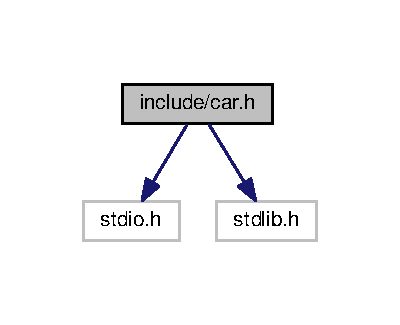
\includegraphics[width=192pt]{car_8h__incl}
\end{center}
\end{figure}
\subsection*{Classes}
\begin{DoxyCompactItemize}
\item 
struct \hyperlink{structcar}{car}
\end{DoxyCompactItemize}
\subsection*{Typedefs}
\begin{DoxyCompactItemize}
\item 
typedef struct \hyperlink{structcar}{car} \hyperlink{car_8h_ac4e92fe9b49abb7e2c4ef2b9c8ae4614}{Car}
\end{DoxyCompactItemize}
\subsection*{Functions}
\begin{DoxyCompactItemize}
\item 
\hyperlink{car_8h_ac4e92fe9b49abb7e2c4ef2b9c8ae4614}{Car} $\ast$ \hyperlink{car_8h_abf29c76dde147a2cb1ddfce3123980c2}{initialize\+Car} (char start\+Point, char end\+Point, double arrive\+Time)
\item 
char \hyperlink{car_8h_a971f248b7d871c57229b33d3a06ad884}{getstart\+Point} (\hyperlink{car_8h_ac4e92fe9b49abb7e2c4ef2b9c8ae4614}{Car} $\ast$\hyperlink{structcar}{car})
\item 
char \hyperlink{car_8h_aec879ec1e8cf846ffb413ad7ed71033d}{getend\+Point} (\hyperlink{car_8h_ac4e92fe9b49abb7e2c4ef2b9c8ae4614}{Car} $\ast$\hyperlink{structcar}{car})
\item 
double \hyperlink{car_8h_a80c4d63204484255e1a8356b984b057e}{getarrive\+Time} (\hyperlink{car_8h_ac4e92fe9b49abb7e2c4ef2b9c8ae4614}{Car} $\ast$\hyperlink{structcar}{car})
\item 
void \hyperlink{car_8h_abe6525d033442d93df5d10952815cbe3}{print\+Car} (void $\ast$to\+Be\+Printed)
\item 
void \hyperlink{car_8h_a37f947dfb59c985765e436386d82b8ee}{delete\+Car} (void $\ast$to\+Be\+Deleted)
\item 
int \hyperlink{car_8h_a00f47305e5583254cb8fa41544525684}{compare\+Cars} (const void $\ast$first, const void $\ast$second)
\item 
void \hyperlink{car_8h_a35a5402b52b553ab2b1f5eac87233c68}{load\+Cars} (char $\ast$filename, Queue $\ast$all\+Cars)
\end{DoxyCompactItemize}


\subsection{Detailed Description}
File containing the function definitions needed for car struct. 

\begin{DoxyAuthor}{Author}
Ralph Arvin De Castro 
\end{DoxyAuthor}
\begin{DoxyDate}{Date}
June 2018 
\end{DoxyDate}


\subsection{Typedef Documentation}
\mbox{\Hypertarget{car_8h_ac4e92fe9b49abb7e2c4ef2b9c8ae4614}\label{car_8h_ac4e92fe9b49abb7e2c4ef2b9c8ae4614}} 
\index{car.\+h@{car.\+h}!Car@{Car}}
\index{Car@{Car}!car.\+h@{car.\+h}}
\subsubsection{\texorpdfstring{Car}{Car}}
{\footnotesize\ttfamily typedef struct \hyperlink{structcar}{car} \hyperlink{car_8h_ac4e92fe9b49abb7e2c4ef2b9c8ae4614}{Car}}

Car. It contains elements which are start\+Point(from N S E or W) and end\+Point(to R F or L) character and an arrival, waiting and intersection(what time they went to the intersection) time of the car. 

\subsection{Function Documentation}
\mbox{\Hypertarget{car_8h_a00f47305e5583254cb8fa41544525684}\label{car_8h_a00f47305e5583254cb8fa41544525684}} 
\index{car.\+h@{car.\+h}!compare\+Cars@{compare\+Cars}}
\index{compare\+Cars@{compare\+Cars}!car.\+h@{car.\+h}}
\subsubsection{\texorpdfstring{compare\+Cars()}{compareCars()}}
{\footnotesize\ttfamily int compare\+Cars (\begin{DoxyParamCaption}\item[{const void $\ast$}]{first,  }\item[{const void $\ast$}]{second }\end{DoxyParamCaption})}

Compares the arrival time of cars \begin{DoxyReturn}{Returns}
integer that determines the comparison of two cars 
\end{DoxyReturn}

\begin{DoxyParams}{Parameters}
{\em first} & void pointer to be casted to an integer \\
\hline
{\em second} & void pointer to be casted to an integer \\
\hline
\end{DoxyParams}
\mbox{\Hypertarget{car_8h_a37f947dfb59c985765e436386d82b8ee}\label{car_8h_a37f947dfb59c985765e436386d82b8ee}} 
\index{car.\+h@{car.\+h}!delete\+Car@{delete\+Car}}
\index{delete\+Car@{delete\+Car}!car.\+h@{car.\+h}}
\subsubsection{\texorpdfstring{delete\+Car()}{deleteCar()}}
{\footnotesize\ttfamily void delete\+Car (\begin{DoxyParamCaption}\item[{void $\ast$}]{to\+Be\+Deleted }\end{DoxyParamCaption})}

Frees the car struct 
\begin{DoxyParams}{Parameters}
{\em to\+Be\+Deleted} & void pointer to be casted to a car type \\
\hline
\end{DoxyParams}
\mbox{\Hypertarget{car_8h_a80c4d63204484255e1a8356b984b057e}\label{car_8h_a80c4d63204484255e1a8356b984b057e}} 
\index{car.\+h@{car.\+h}!getarrive\+Time@{getarrive\+Time}}
\index{getarrive\+Time@{getarrive\+Time}!car.\+h@{car.\+h}}
\subsubsection{\texorpdfstring{getarrive\+Time()}{getarriveTime()}}
{\footnotesize\ttfamily double getarrive\+Time (\begin{DoxyParamCaption}\item[{\hyperlink{car_8h_ac4e92fe9b49abb7e2c4ef2b9c8ae4614}{Car} $\ast$}]{car }\end{DoxyParamCaption})}

Gets the arrive\+Time of the car \begin{DoxyReturn}{Returns}
arrival time of the car 
\end{DoxyReturn}

\begin{DoxyParams}{Parameters}
{\em car} & pointer to a car struct \\
\hline
\end{DoxyParams}
\mbox{\Hypertarget{car_8h_aec879ec1e8cf846ffb413ad7ed71033d}\label{car_8h_aec879ec1e8cf846ffb413ad7ed71033d}} 
\index{car.\+h@{car.\+h}!getend\+Point@{getend\+Point}}
\index{getend\+Point@{getend\+Point}!car.\+h@{car.\+h}}
\subsubsection{\texorpdfstring{getend\+Point()}{getendPoint()}}
{\footnotesize\ttfamily char getend\+Point (\begin{DoxyParamCaption}\item[{\hyperlink{car_8h_ac4e92fe9b49abb7e2c4ef2b9c8ae4614}{Car} $\ast$}]{car }\end{DoxyParamCaption})}

Gets the end direction of the car \begin{DoxyReturn}{Returns}
character end\+Point R F L 
\end{DoxyReturn}

\begin{DoxyParams}{Parameters}
{\em car} & pointer to a car struct \\
\hline
\end{DoxyParams}
\mbox{\Hypertarget{car_8h_a971f248b7d871c57229b33d3a06ad884}\label{car_8h_a971f248b7d871c57229b33d3a06ad884}} 
\index{car.\+h@{car.\+h}!getstart\+Point@{getstart\+Point}}
\index{getstart\+Point@{getstart\+Point}!car.\+h@{car.\+h}}
\subsubsection{\texorpdfstring{getstart\+Point()}{getstartPoint()}}
{\footnotesize\ttfamily char getstart\+Point (\begin{DoxyParamCaption}\item[{\hyperlink{car_8h_ac4e92fe9b49abb7e2c4ef2b9c8ae4614}{Car} $\ast$}]{car }\end{DoxyParamCaption})}

Gets the starting direction of the car \begin{DoxyReturn}{Returns}
character start\+Point N S E W 
\end{DoxyReturn}

\begin{DoxyParams}{Parameters}
{\em car} & pointer to a car struct \\
\hline
\end{DoxyParams}
\mbox{\Hypertarget{car_8h_abf29c76dde147a2cb1ddfce3123980c2}\label{car_8h_abf29c76dde147a2cb1ddfce3123980c2}} 
\index{car.\+h@{car.\+h}!initialize\+Car@{initialize\+Car}}
\index{initialize\+Car@{initialize\+Car}!car.\+h@{car.\+h}}
\subsubsection{\texorpdfstring{initialize\+Car()}{initializeCar()}}
{\footnotesize\ttfamily \hyperlink{car_8h_ac4e92fe9b49abb7e2c4ef2b9c8ae4614}{Car}$\ast$ initialize\+Car (\begin{DoxyParamCaption}\item[{char}]{start\+Point,  }\item[{char}]{end\+Point,  }\item[{double}]{arrive\+Time }\end{DoxyParamCaption})}

Function to allocate memory to the car, set proper data to its members \begin{DoxyReturn}{Returns}
pointer to the car 
\end{DoxyReturn}

\begin{DoxyParams}{Parameters}
{\em start\+Point} & character N S E W or direction of where the car was coming from \\
\hline
{\em end\+Point} & character R F L or direction of the car is going to \\
\hline
{\em arrive\+Time} & time that the car arrives in the queue \\
\hline
\end{DoxyParams}
\mbox{\Hypertarget{car_8h_a35a5402b52b553ab2b1f5eac87233c68}\label{car_8h_a35a5402b52b553ab2b1f5eac87233c68}} 
\index{car.\+h@{car.\+h}!load\+Cars@{load\+Cars}}
\index{load\+Cars@{load\+Cars}!car.\+h@{car.\+h}}
\subsubsection{\texorpdfstring{load\+Cars()}{loadCars()}}
{\footnotesize\ttfamily void load\+Cars (\begin{DoxyParamCaption}\item[{char $\ast$}]{filename,  }\item[{Queue $\ast$}]{all\+Cars }\end{DoxyParamCaption})}

Parse file and put car data in a queue 
\begin{DoxyParams}{Parameters}
{\em filename} & name of the file that has the data \\
\hline
{\em all\+Cars} & pointer to a queue where all the car data will be enqueued \\
\hline
\end{DoxyParams}
\mbox{\Hypertarget{car_8h_abe6525d033442d93df5d10952815cbe3}\label{car_8h_abe6525d033442d93df5d10952815cbe3}} 
\index{car.\+h@{car.\+h}!print\+Car@{print\+Car}}
\index{print\+Car@{print\+Car}!car.\+h@{car.\+h}}
\subsubsection{\texorpdfstring{print\+Car()}{printCar()}}
{\footnotesize\ttfamily void print\+Car (\begin{DoxyParamCaption}\item[{void $\ast$}]{to\+Be\+Printed }\end{DoxyParamCaption})}

Prints the elements of the car 
\begin{DoxyParams}{Parameters}
{\em to\+Be\+Printed} & void pointer to be casted to a car type \\
\hline
\end{DoxyParams}

%--- End generated contents ---

% Index
\backmatter
\newpage
\phantomsection
\clearemptydoublepage
\addcontentsline{toc}{chapter}{Index}
\printindex

\end{document}
